\section{Índices de governo eletrônico}

Existem 4 tipos de índices de governo eletrônico, segundo \cite{martinez2022egovernment}: EDGI da ONU, GTMI do Banco Mundial, DESI da Comissão Europeia da União Europeia e DGI da OECD.

O DESI não será usado porque o índice, administrado pela Comissão Europeia da UE, foca no análise individual de cada estado-membro da UE para que eles possam identificar áreas que precisam de ações prioritárias e capítulos temáticos que providenciam analises a nível supranacional em áreas de áreas chave de política digital \cite{desi_2022}.

\subsection{EGDI}

% DEFINIR O QUE EGDI

\subsubsection{Coeficiente de correlação de Pearson: EGDI, índice de democracia eleitoral, PIB \textit{per capital} e uso de internet}

Ao analisar os dados do \href{https://publicadministration.un.org/egovkb/en-us/About/Overview/-E-Government-Development-Index}{EGDI}, foi notado que tanto democracias consolidade, quanto autocracias históricas tem um EGDI alto. O critério para entender quais paises são democráticos ou autocráticos foram as figuras presentes no Apêndice \ref{demo_auto_mundo}. 

Nota-se que em qualquer figura o Brasil é considerado uma democrácia (eleitoral, completa ou liberal), estão na minoria númerica de países democráticas (88), conforme exposto por \cite{nord2025democracy}, contra 91 autocracias.

Outro fator chamou atenção: há EGDI alto em paises tanto autocráticos, quanto democráticos que têm PIB \textit{per capita} alto, conforme comparação dos \href{https://data.worldbank.org/indicator/NY.GDP.PCAP.PP.KD}{com o PIB \textit{per capita} dos paises}. 

Além disso, percebeu-se que em paises tanto autocráticos, quanto democráticos, o uso de internet é alto quando comparados os dados do \href{https://datahub.itu.int/data/?e=701&i=11624&c=701}{uso individual de internet no mundo} pelo ITU.

Em razão disso, um questionamento surgiu: qual é relação entre EDGI e índice de democracia eleitoral do \href{https://www.v-dem.net/}{V-Dem}, o PIB \textit{per capita} e uso de internet tanto nos páises do mundo, quanto no Brasil. Para responder a pergunta, foi usado o coeficiente de correlação de Pearson. O resultado foi dividido nas figuras \ref{fig:correlacao3}, \ref{fig:correlacao4}, \ref{fig:correlacao5}, \ref{fig:correlacao8}, \ref{fig:correlacao6} e \ref{fig:correlacao7}.

\begin{figure}[H]
    \centering
    \caption{Coeficiente de correlação de Pearson: índice de democracia eleitoral e o EGDI dos 193 países}
    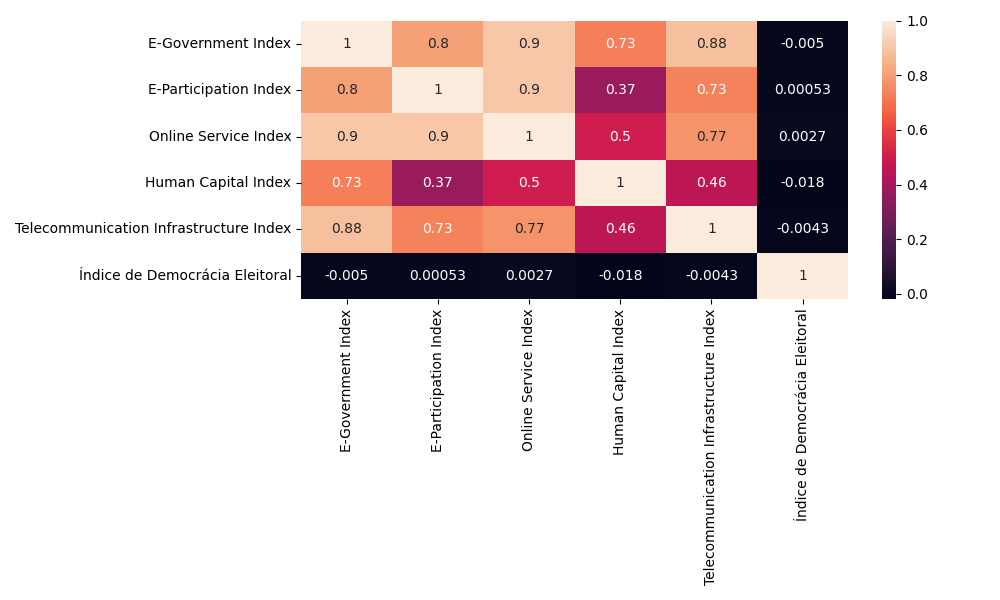
\includegraphics[width=1\linewidth]{figuras/egdi/correlacao3.png}
    \label{fig:correlacao3}
    \footnotesize{Fonte: baseado em \cite{ONU_edgi_mapa} e \cite{electoral_democracy_index}.}
\end{figure}

\begin{figure}[H]
    \centering
    \caption{Coeficiente de correlação de Pearson: PIB \textit{per capita} PPC em USD e EGDI dos 193 países}
    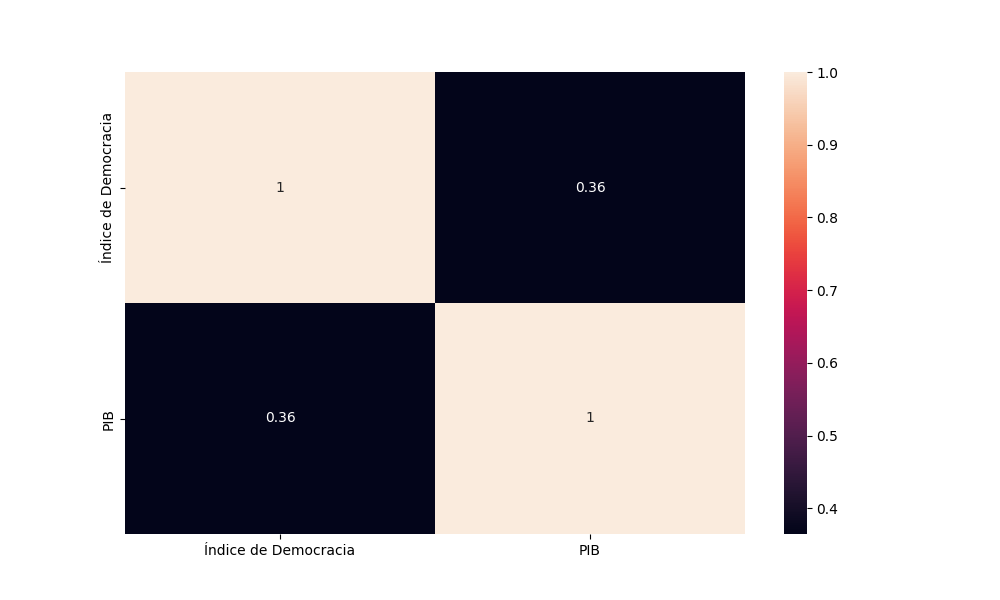
\includegraphics[width=1\linewidth]{figuras/egdi/correlacao4.png}
    \label{fig:correlacao4}
    \footnotesize{Fonte: baseado em \cite{ONU_edgi_mapa} e \cite{WB_pib_per_capita_paises}.}
\end{figure}

\begin{figure}[H]
    \centering
    \caption{Coeficiente de correlação de Pearson: uso de internet e o EGDI \textit{per capita} dos 193 países}
    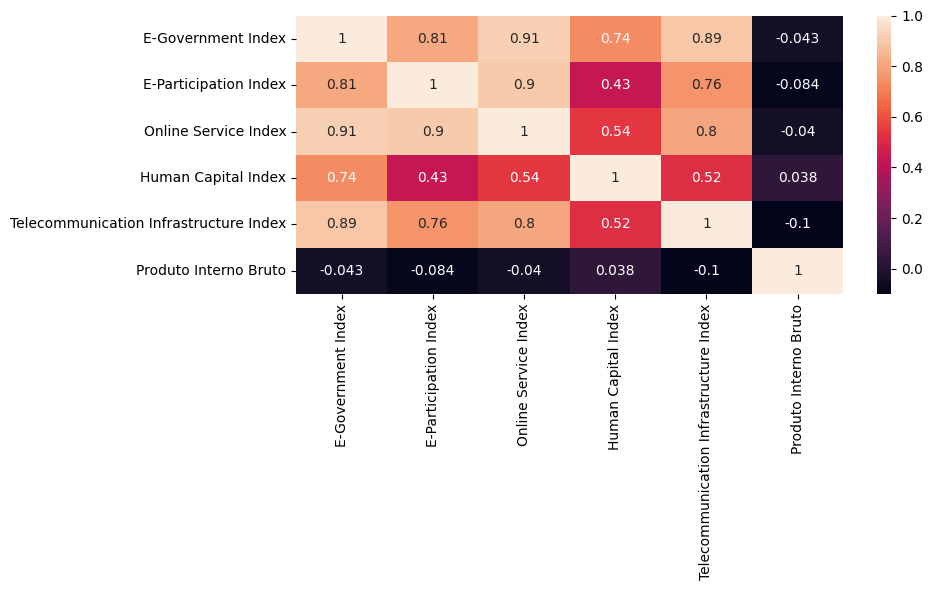
\includegraphics[width=1\linewidth]{figuras/egdi/correlacao5.png}
    \label{fig:correlacao5}
    \footnotesize{Fonte: baseado em \cite{ONU_edgi_mapa} e \cite{ITU_uso_internet_mundo}.}
\end{figure}

\begin{figure}[H]
    \centering
    \caption{Coeficiente de correlação de Pearson: índice de democracia eleitoral e o EGDI do Brasil}
    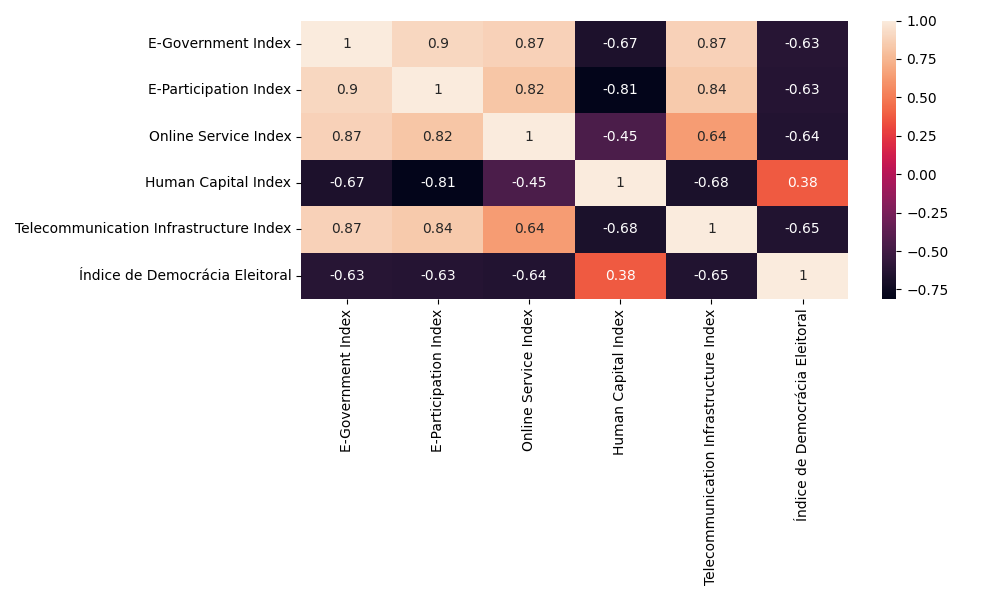
\includegraphics[width=1\linewidth]{figuras/egdi/correlacao8.png}
    \label{fig:correlacao8}
    \footnotesize{Fonte: baseado em \cite{ONU_edgi_mapa} e \cite{electoral_democracy_index}.}
\end{figure}

\begin{figure}[H]
    \centering
    \caption{Coeficiente de correlação de Pearson: PIB \textit{per capita} PPC em USD e EGDI do Brasil}
    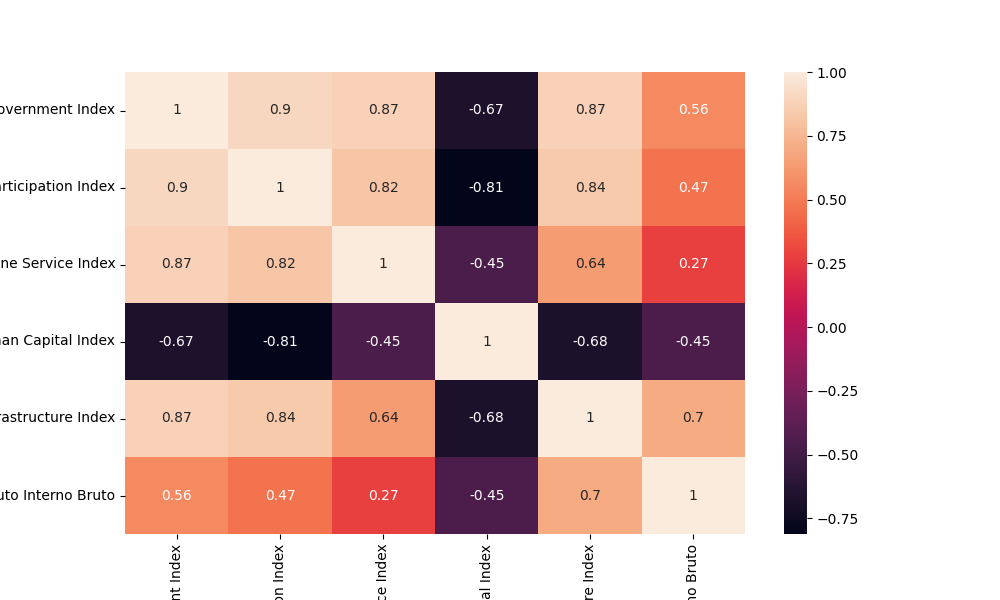
\includegraphics[width=1\linewidth]{figuras/egdi/correlacao6.png}
    \label{fig:correlacao6}
    \footnotesize{Fonte: baseado em \cite{ONU_edgi_mapa} e \cite{WB_pib_per_capita_paises}.}
\end{figure}

\begin{figure}[H]
    \centering
    \caption{Coeficiente de correlação de Pearson: uso de internet e o EGDI}
    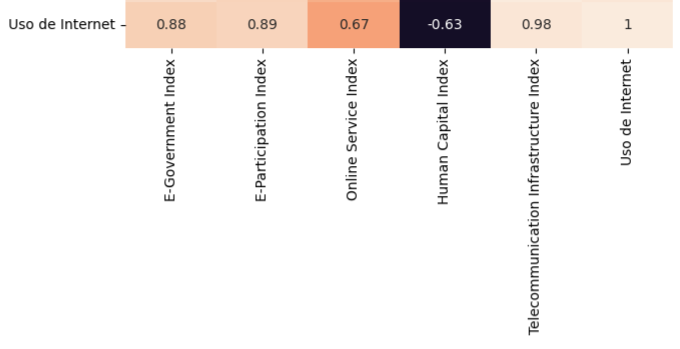
\includegraphics[width=1\linewidth]{figuras/egdi/correlacao7.png}
    \label{fig:correlacao7}
    \footnotesize{Fonte: baseado em \cite{ONU_edgi_mapa} e \cite{ITU_uso_internet_mundo}.}
\end{figure}

%%%%%%%%%%%%

\begin{figure}[H]
    \centering
    \caption{E-Government Index global}
    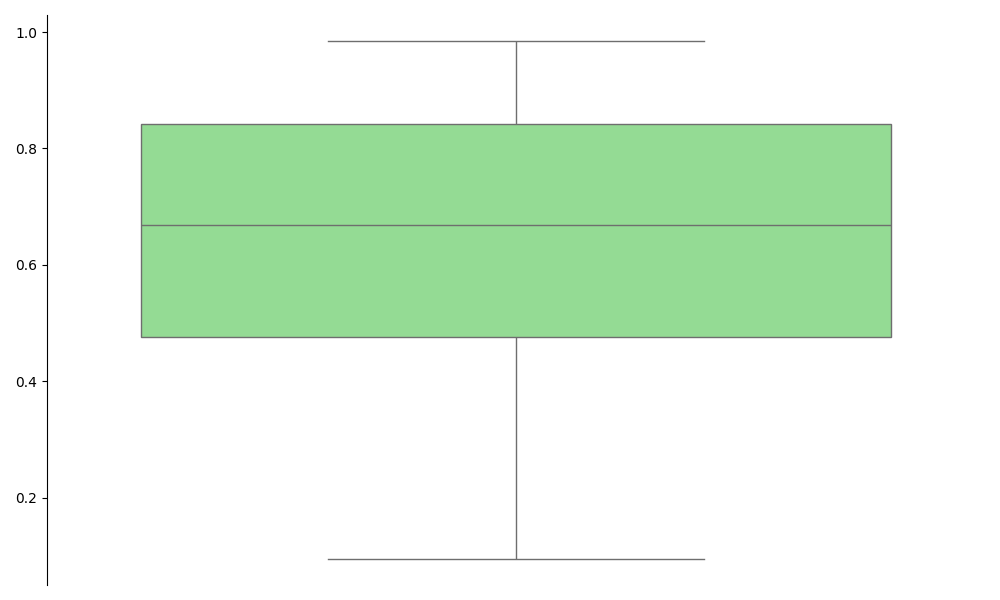
\includegraphics[width=1\linewidth]{figuras/egdi/boxplot_egov_global.png}
    \label{fig:boxplot_egov_global}
    \footnotesize{Fonte: baseado em \cite{ONU_edgi_mapa}.}
\end{figure}

\begin{figure}[H]
    \centering
    \caption{E-Participation Index global}
    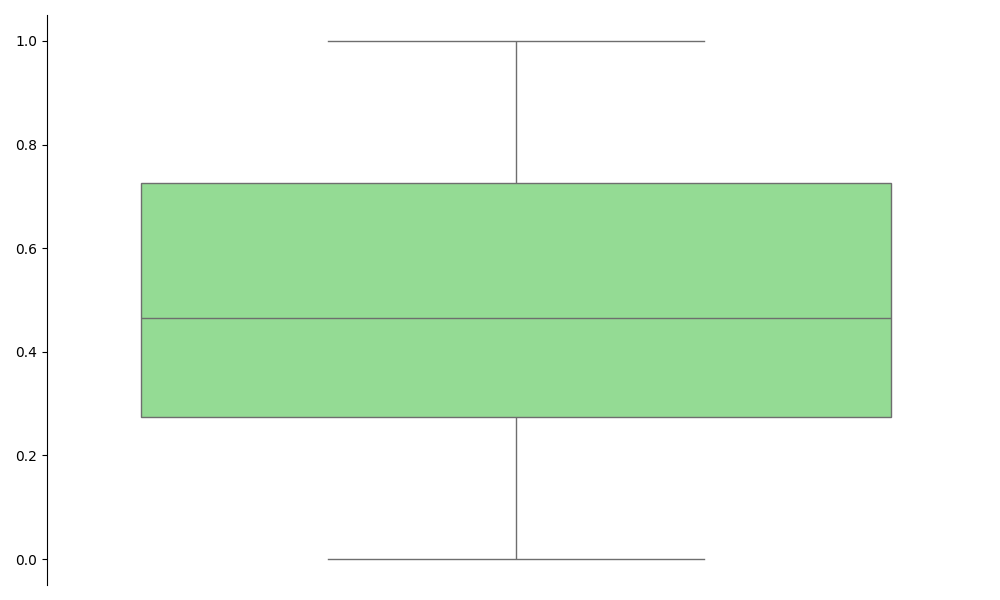
\includegraphics[width=1\linewidth]{figuras/egdi/boxplot_epart_global.png}
    \label{fig:boxplot_epart_global}
    \footnotesize{Fonte: baseado em \cite{ONU_edgi_mapa}.}
\end{figure}

\begin{figure}[H]
    \centering
    \caption{Online Service Index global}
    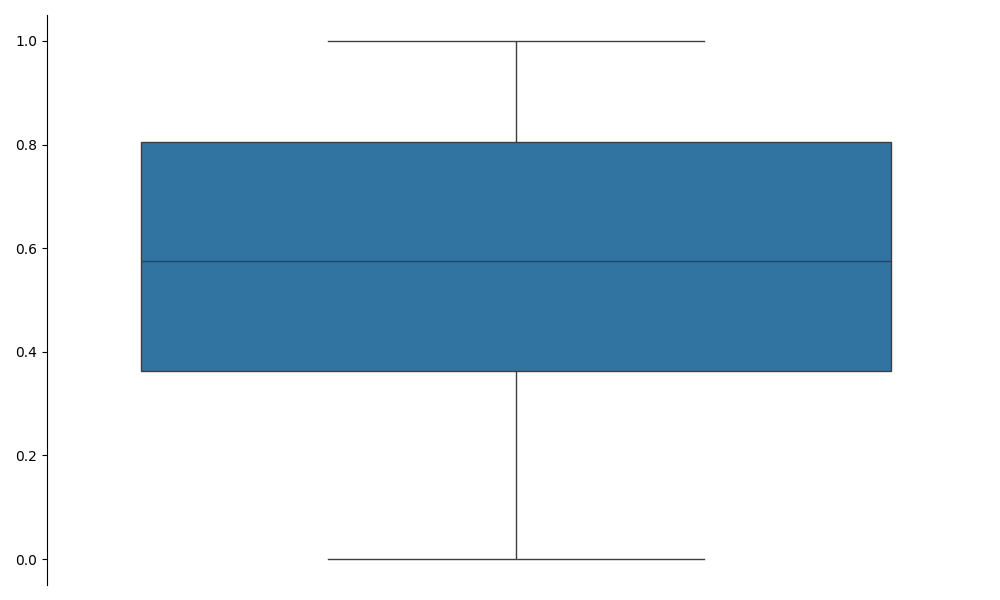
\includegraphics[width=1\linewidth]{figuras/egdi/boxplot_osi_global.png}
    \label{fig:boxplot_osi_global}
    \footnotesize{Fonte: baseado em \cite{ONU_edgi_mapa}.}
\end{figure}

\begin{figure}[H]
    \centering
    \caption{Human Capital Index global}
    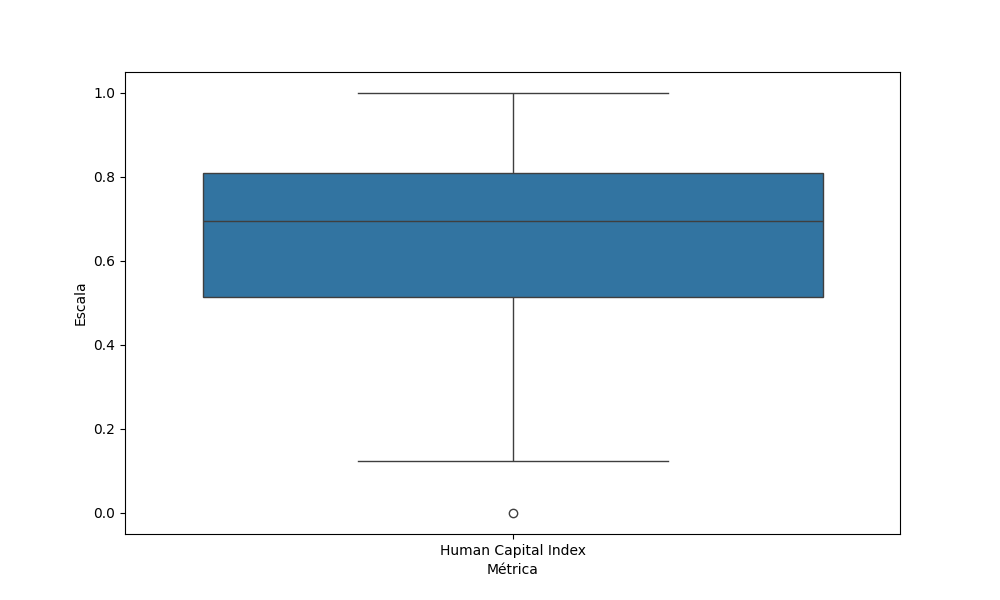
\includegraphics[width=1\linewidth]{figuras/egdi/boxplot_hci_global.png}
    \label{fig:boxplot_hci_global}
    \footnotesize{Fonte: baseado em \cite{ONU_edgi_mapa}.}
\end{figure}

\begin{figure}[H]
    \centering
    \caption{Telecommunication Infrastructure Index global}
    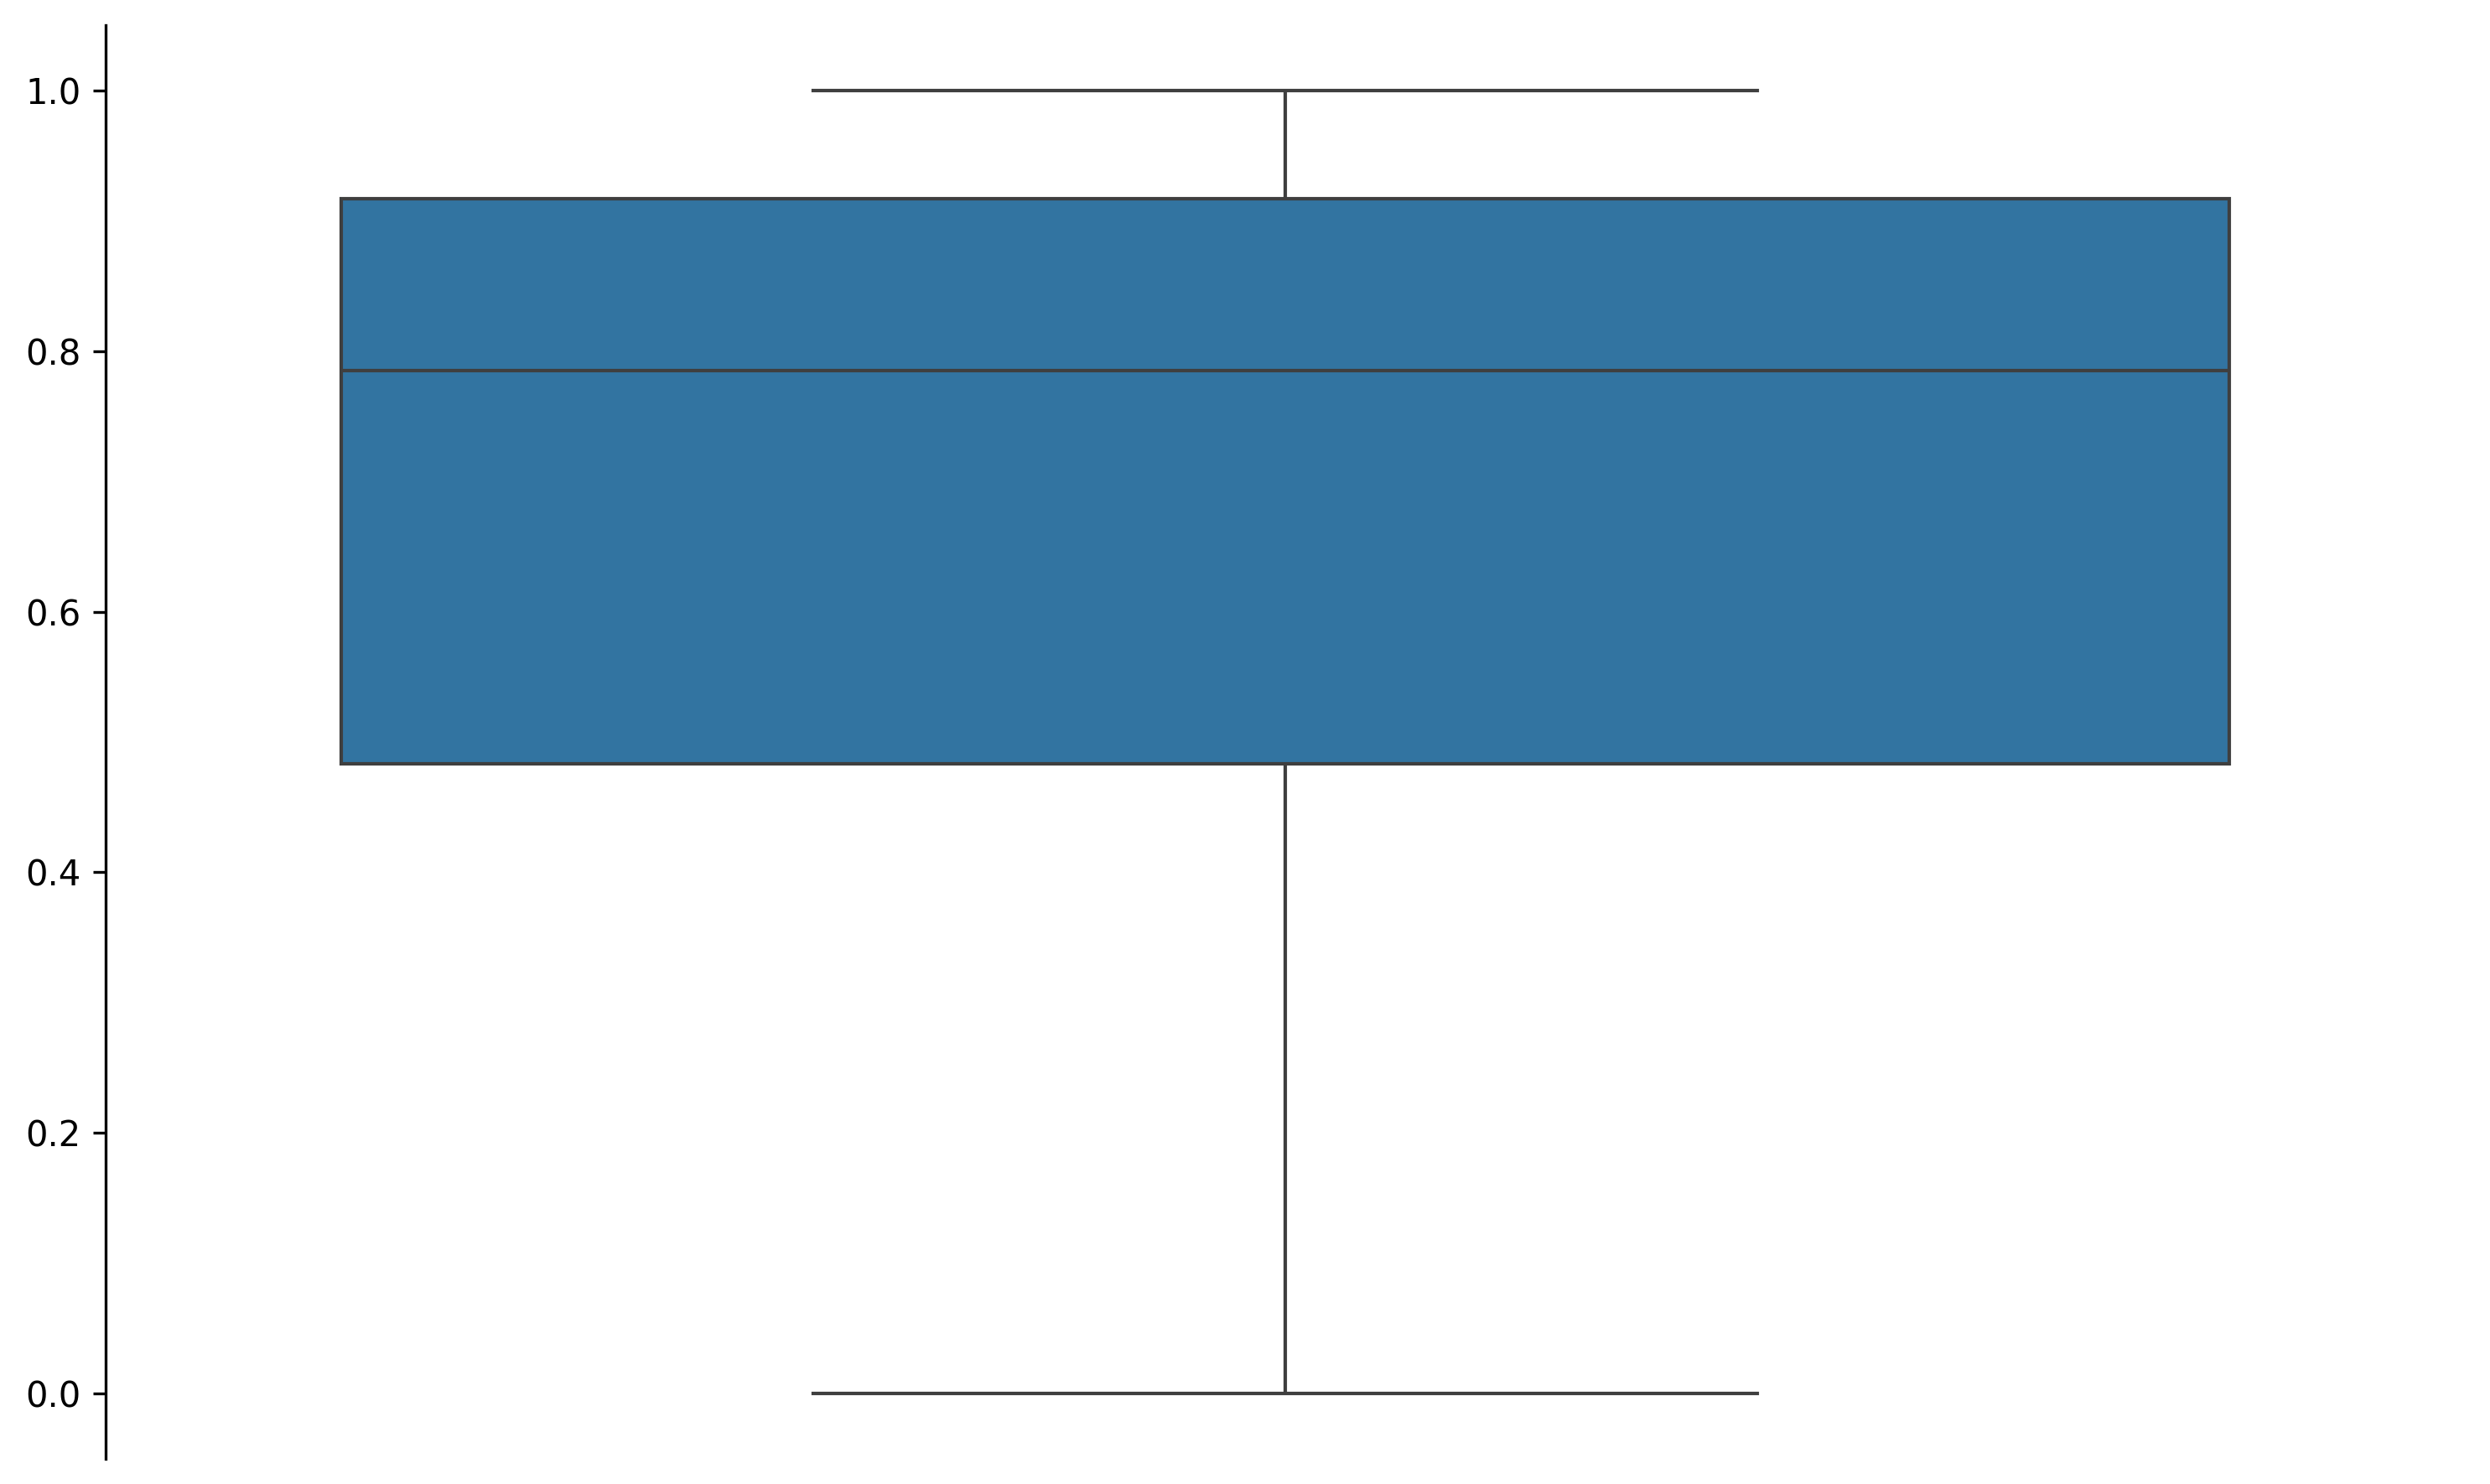
\includegraphics[width=1\linewidth]{figuras/egdi/boxplot_tci_global.png}
    \label{fig:boxplot_tci_global}
    \footnotesize{Fonte: baseado em \cite{ONU_edgi_mapa}.}
\end{figure}

%%%%%%%%%%%%%

\begin{figure}[H]
    \centering
    \caption{Evolução do EGDI do Brasil}
    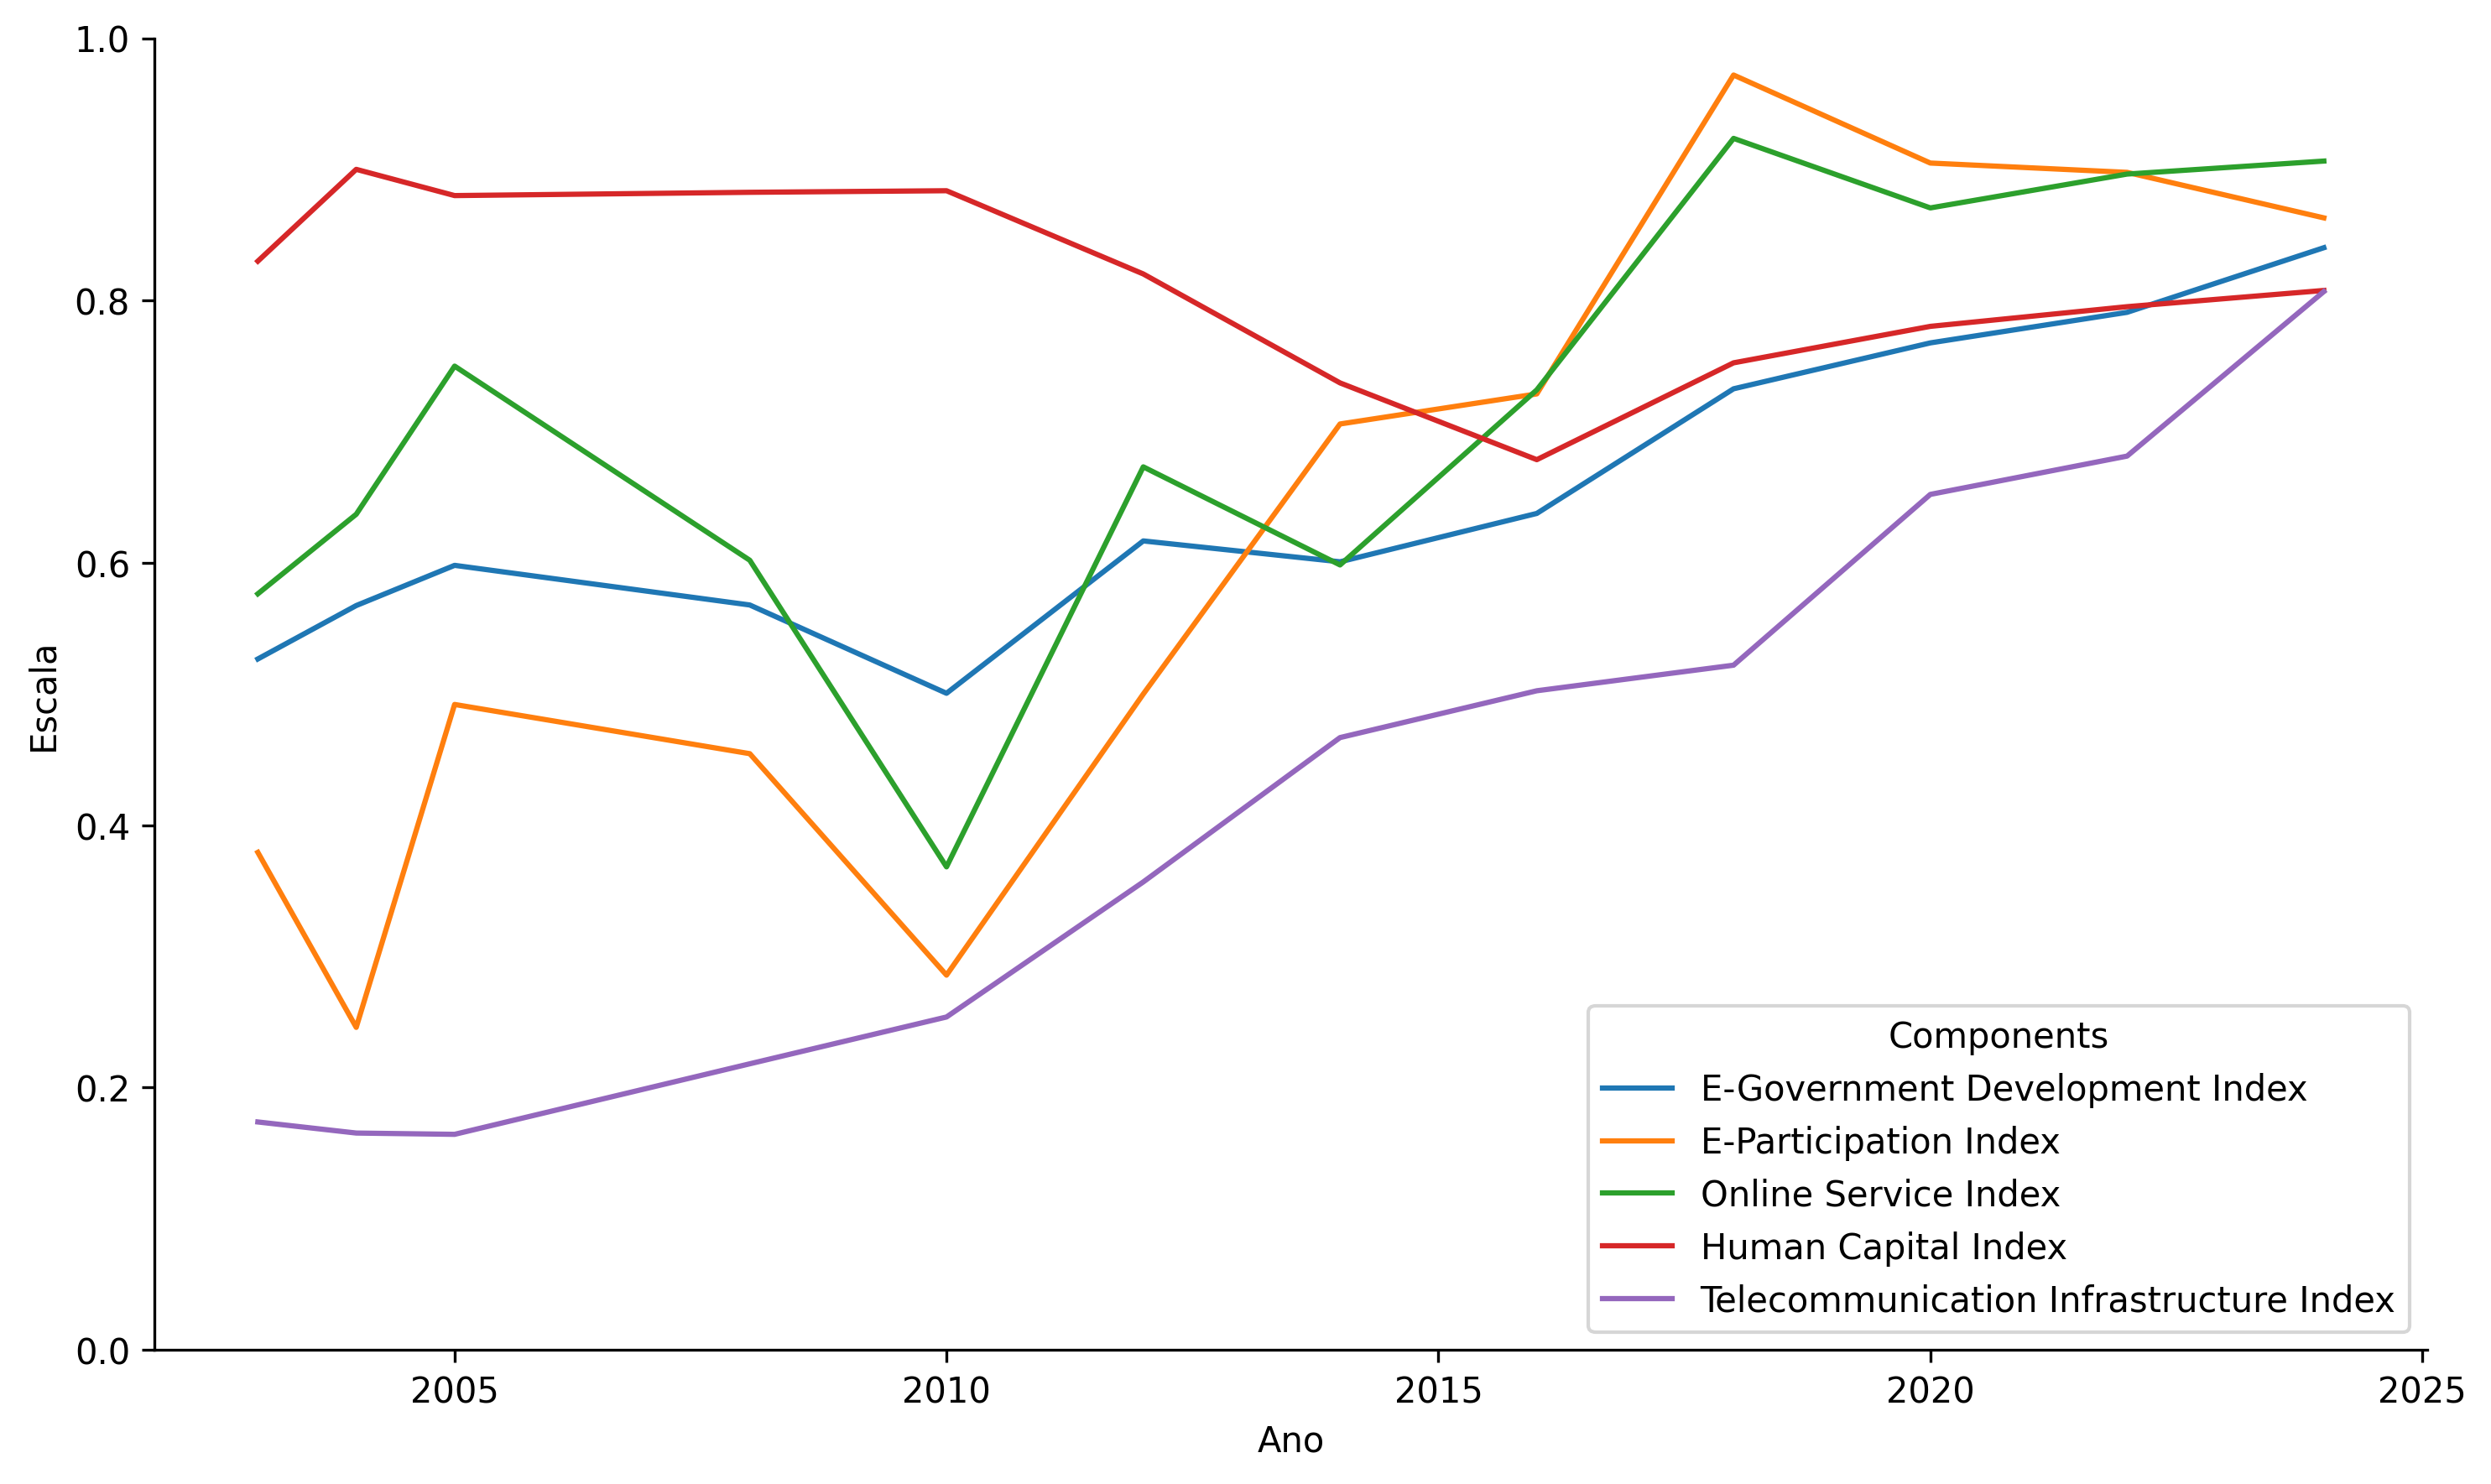
\includegraphics[width=1\linewidth]{figuras/egdi/lineplot_egdi_brasil.png}
    \label{fig:lineplot_egdi_brasil}
    \footnotesize{Fonte: baseado em \cite{ONU_edgi_mapa}.}
\end{figure}

\begin{figure}[H]
    \centering
    \caption{EGDI do Brasil: E-Government Index}
    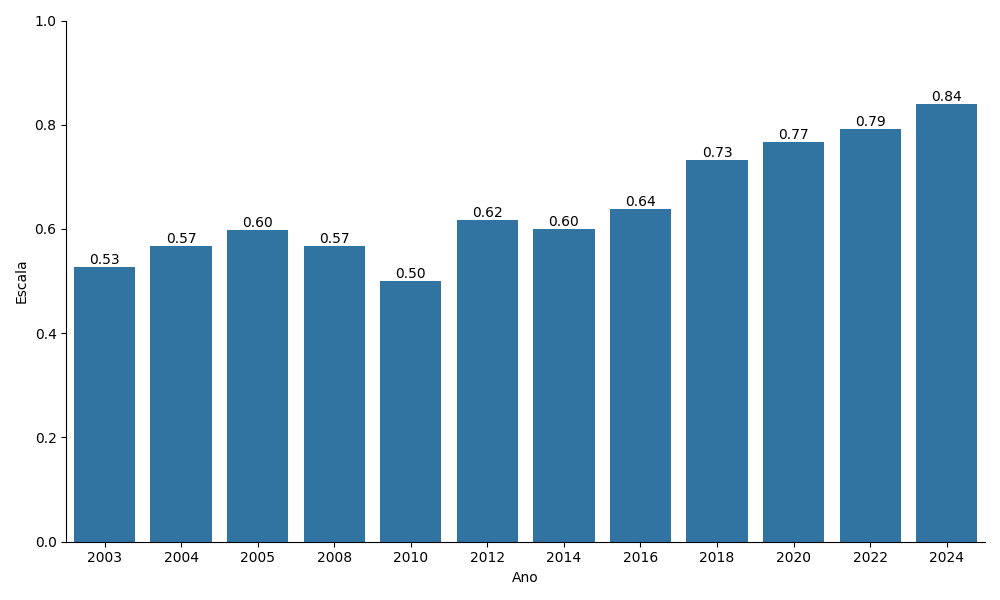
\includegraphics[width=1\linewidth]{figuras/egdi/egdi_brasil_egov.png}
    \label{fig:egdi_brasil_egov}
    \footnotesize{Fonte: baseado em \cite{ONU_edgi_mapa}.}
\end{figure}

\begin{figure}[H]
    \centering
    \caption{EGDI do Brasil: E-Participation Index}
    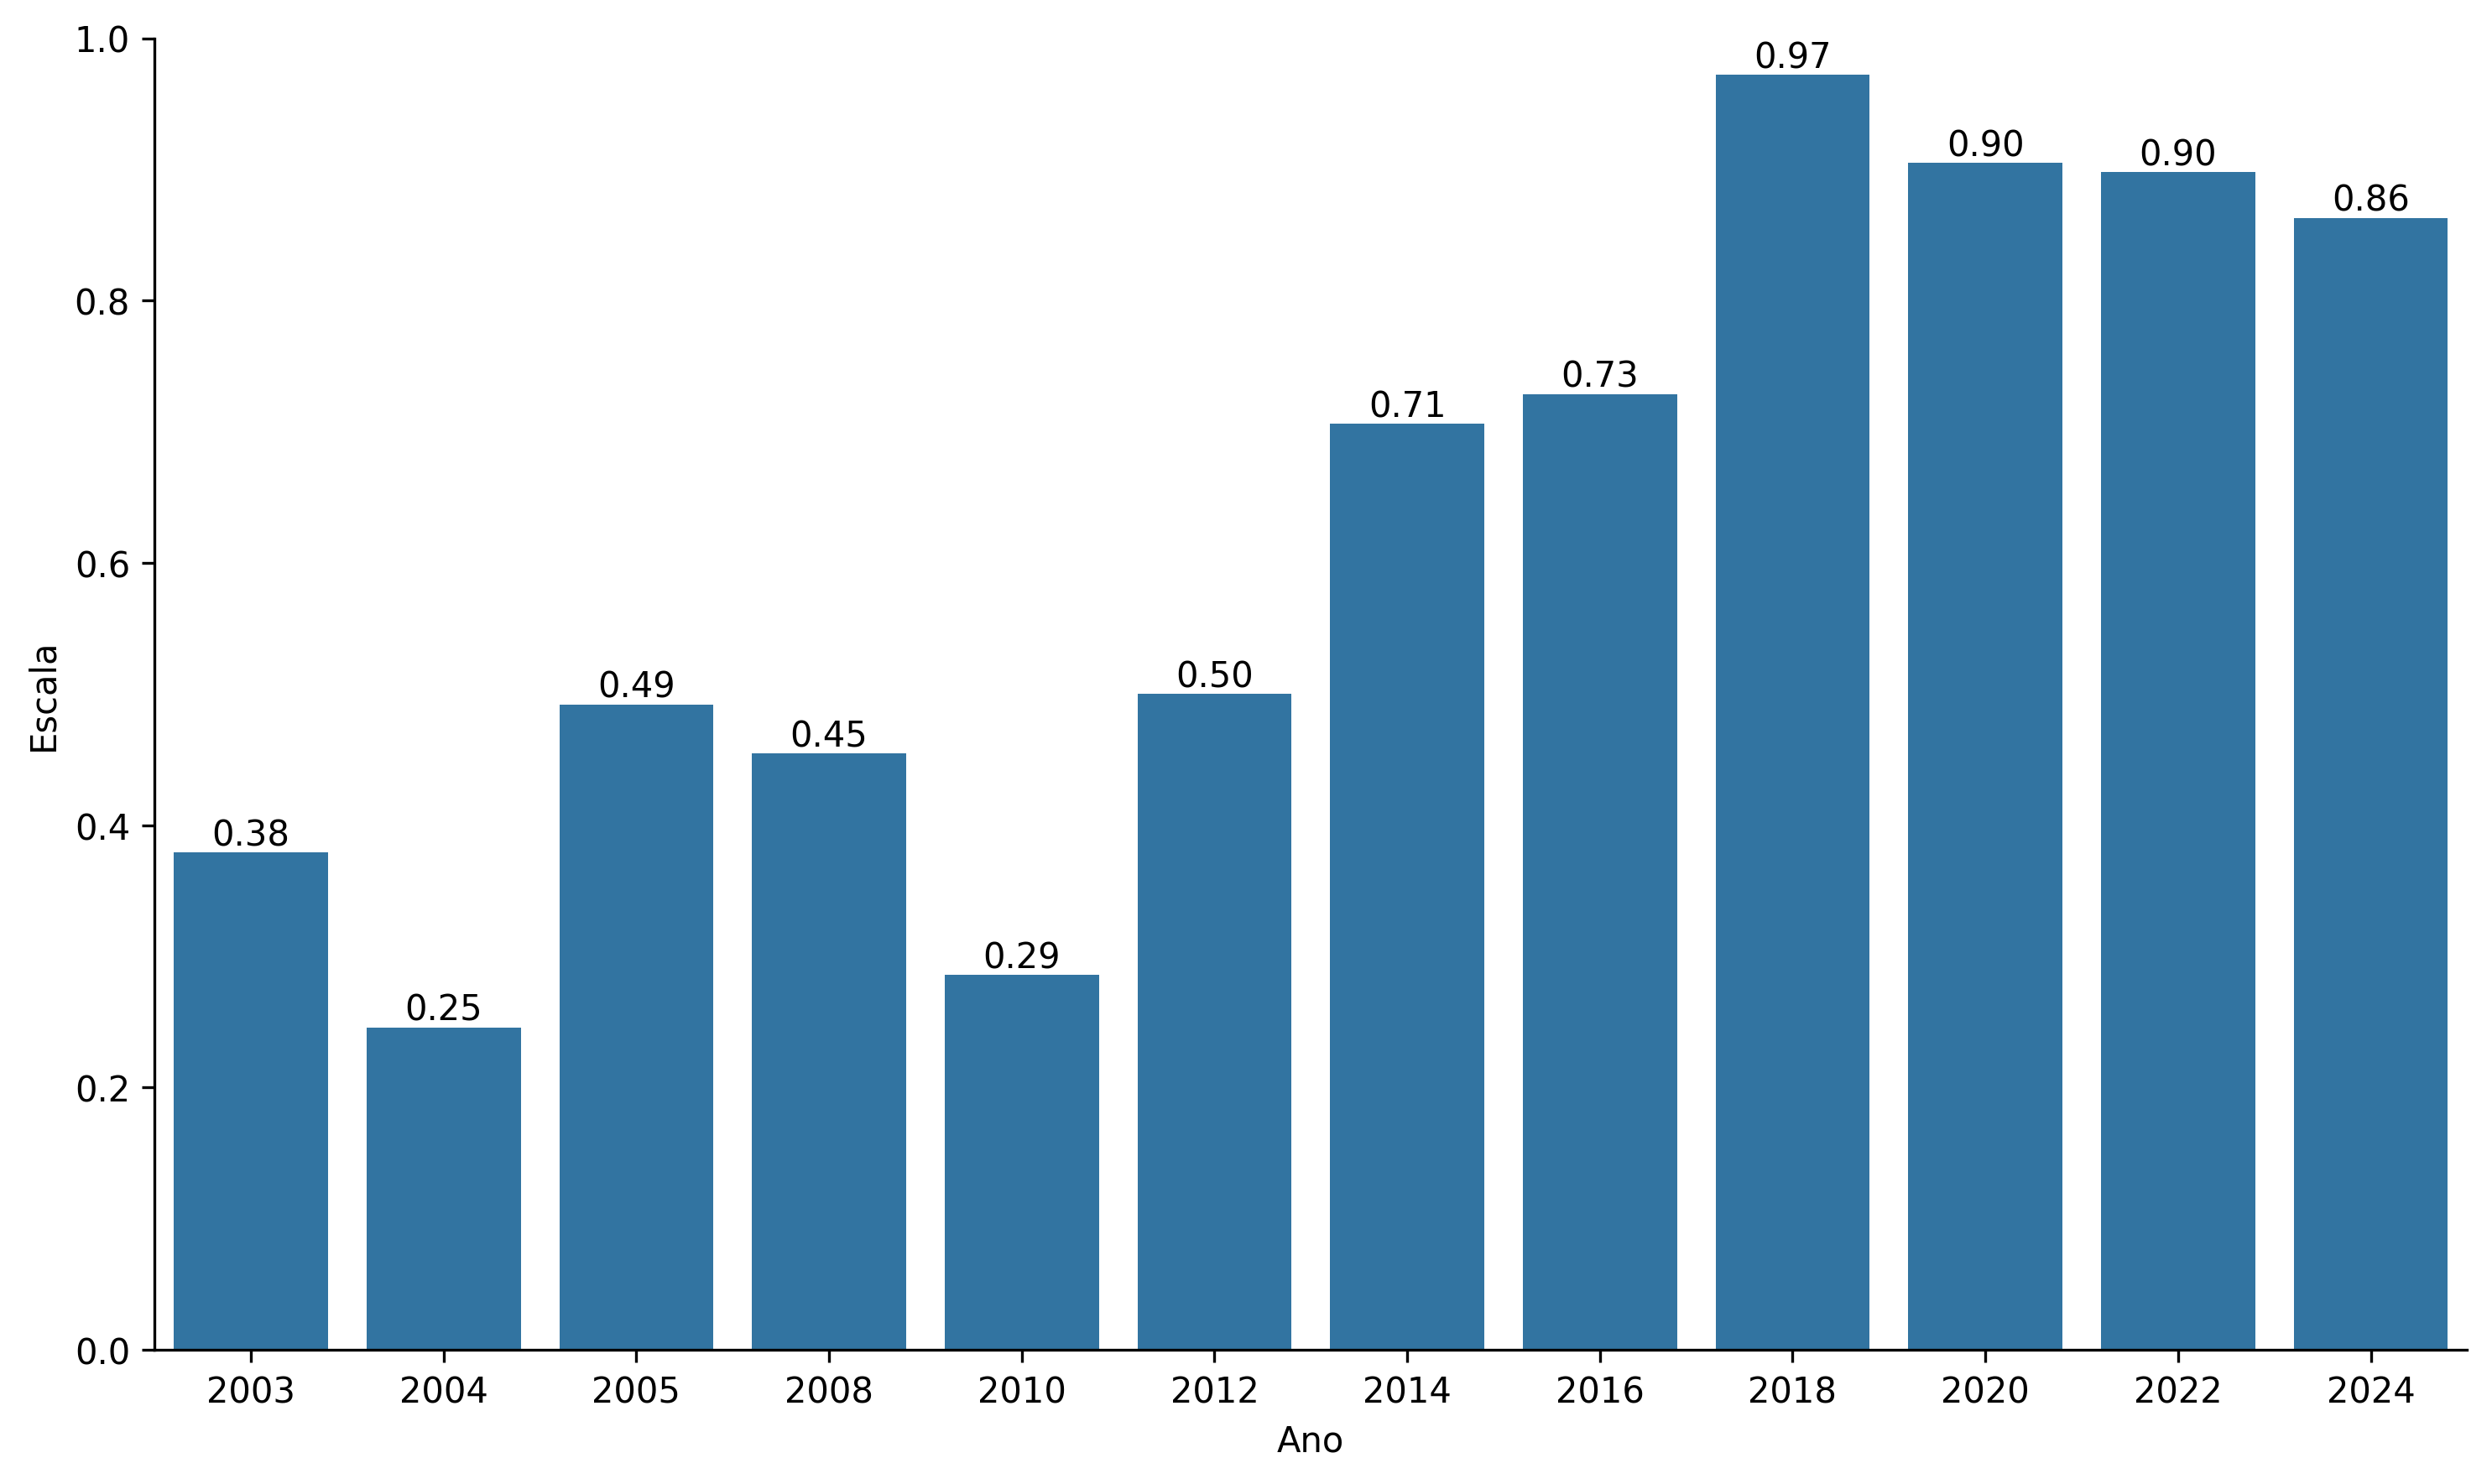
\includegraphics[width=1\linewidth]{figuras/egdi/egdi_brasil_epart.png}
    \label{fig:egdi_brasil_epart}
    \footnotesize{Fonte: baseado em \cite{ONU_edgi_mapa}.}
\end{figure}

\begin{figure}[H]
    \centering
    \caption{EGDI do Brasil: Online Service Index}
    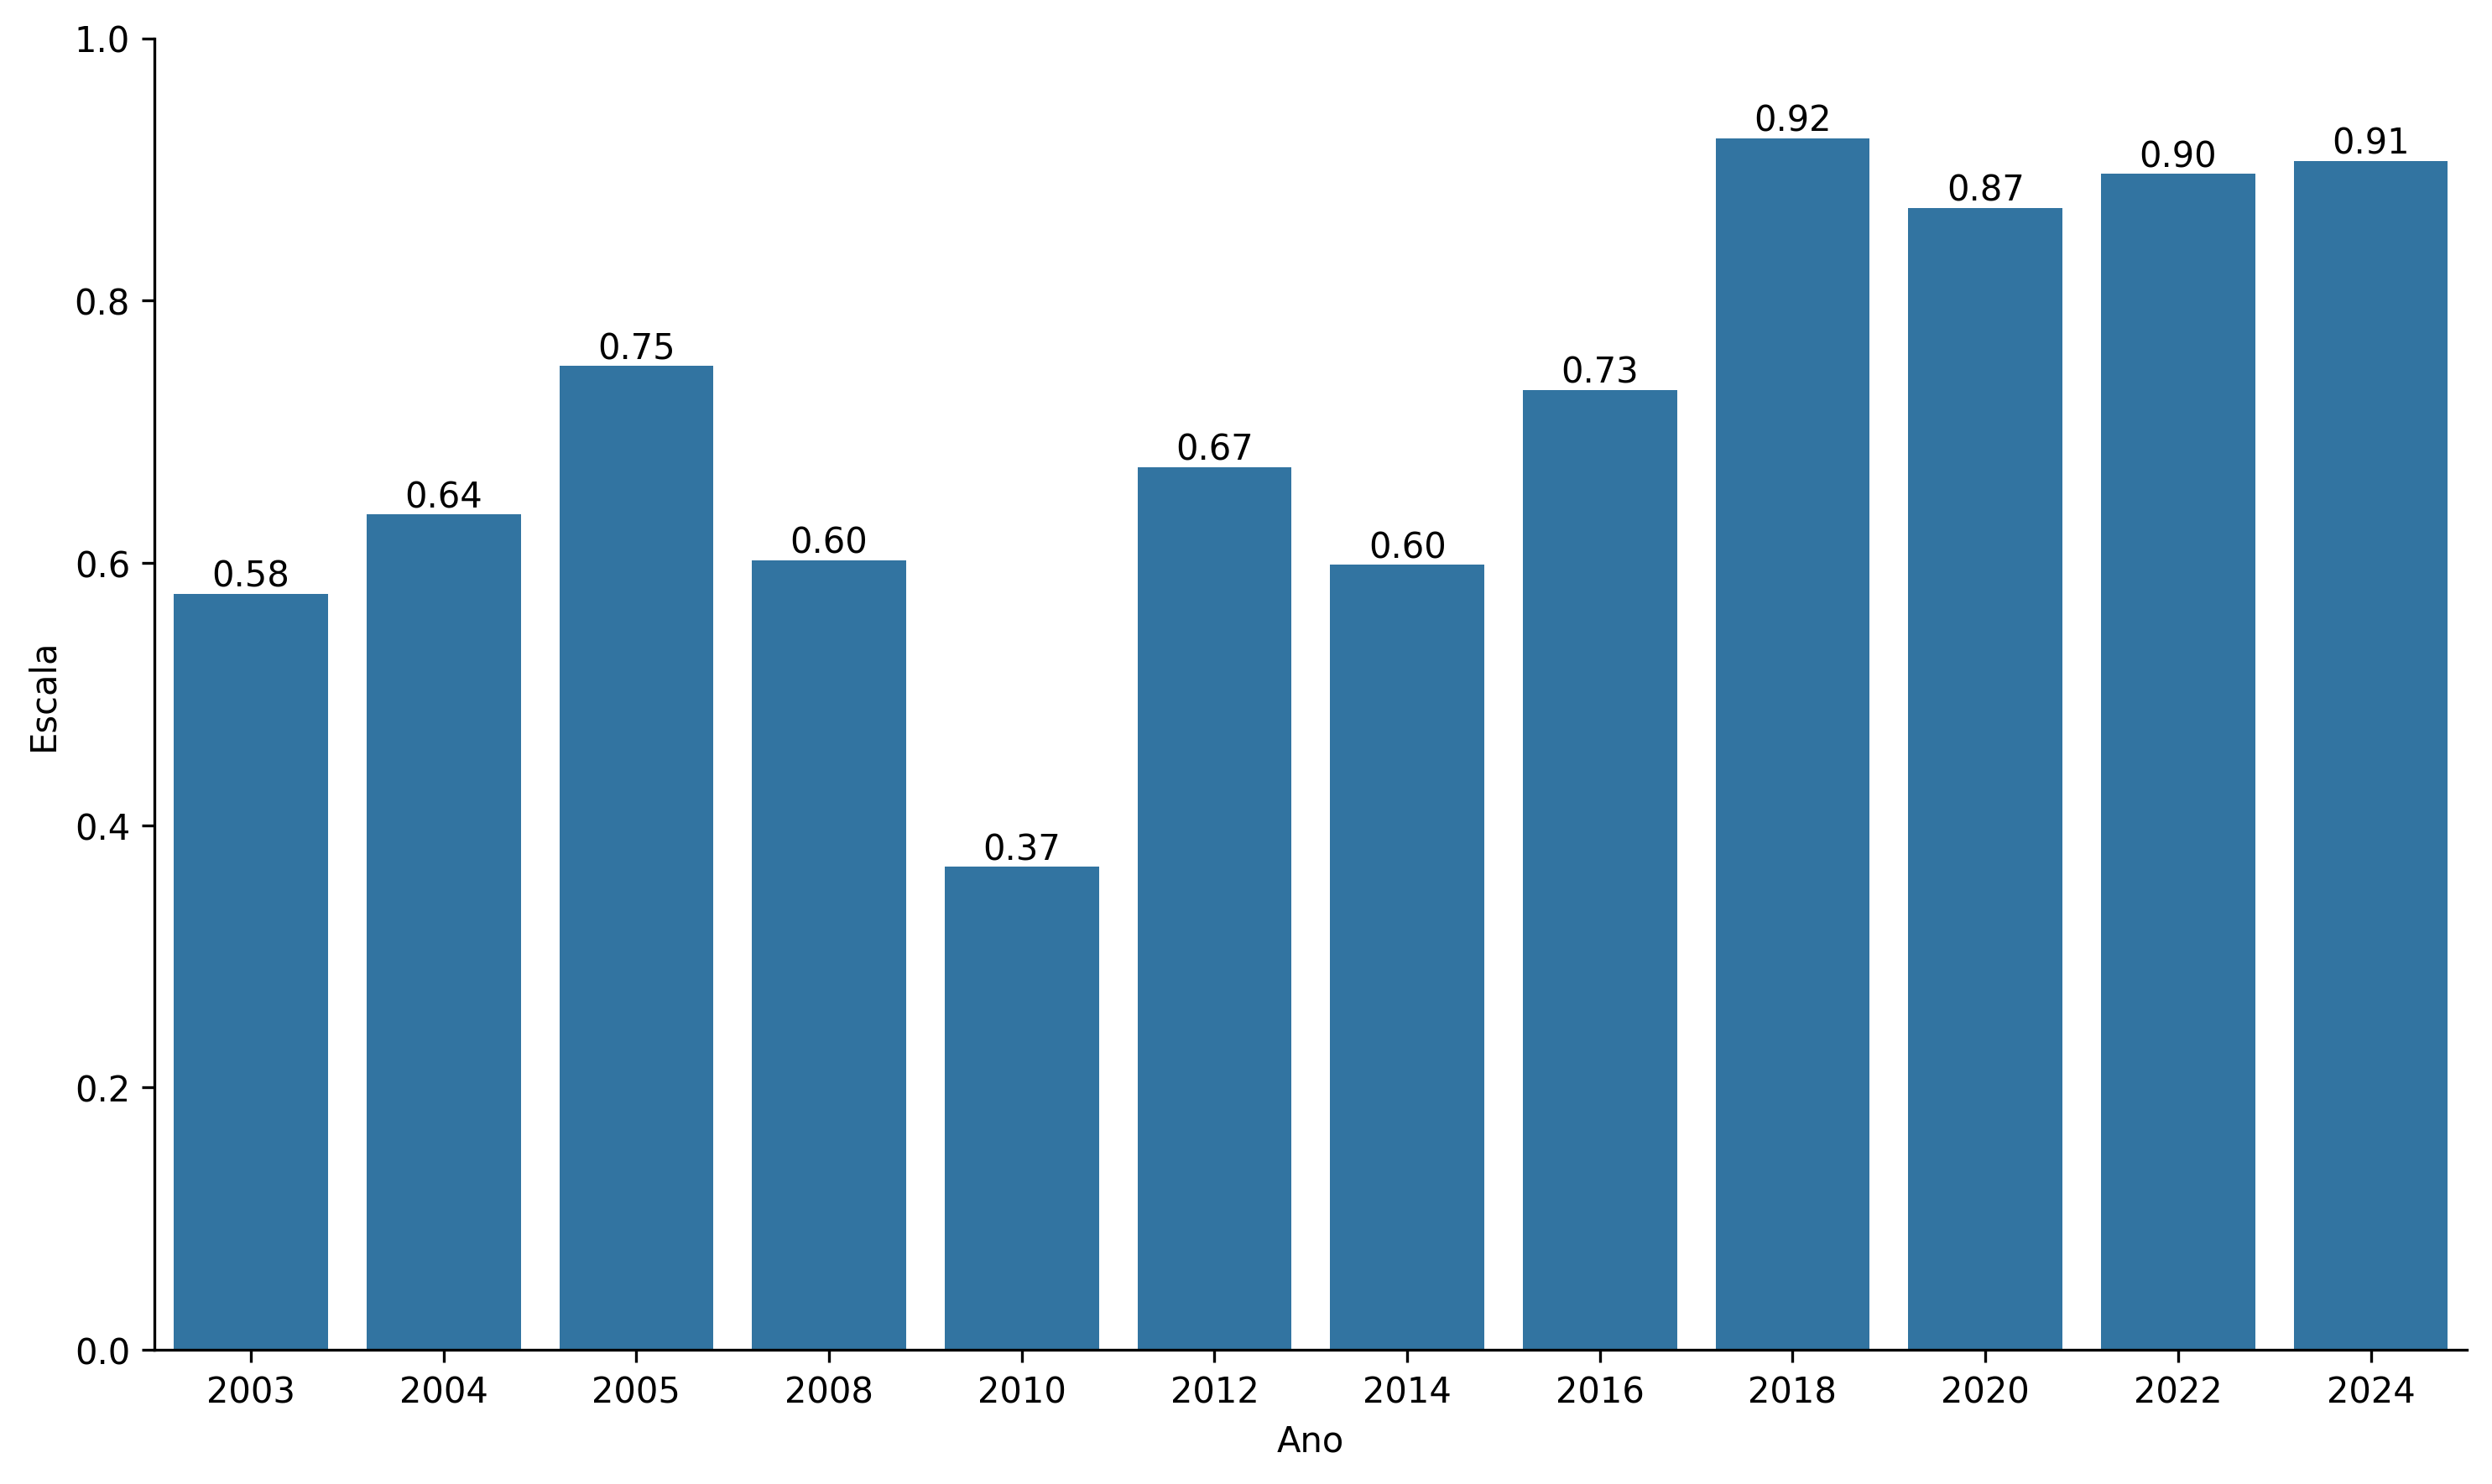
\includegraphics[width=1\linewidth]{figuras/egdi/egdi_brasil_osi.png}
    \label{fig:egdi_brasil_osi}
    \footnotesize{Fonte: baseado em \cite{ONU_edgi_mapa}.}
\end{figure}

\begin{figure}[H]
    \centering
    \caption{EGDI do Brasil: Human Capital Index}
    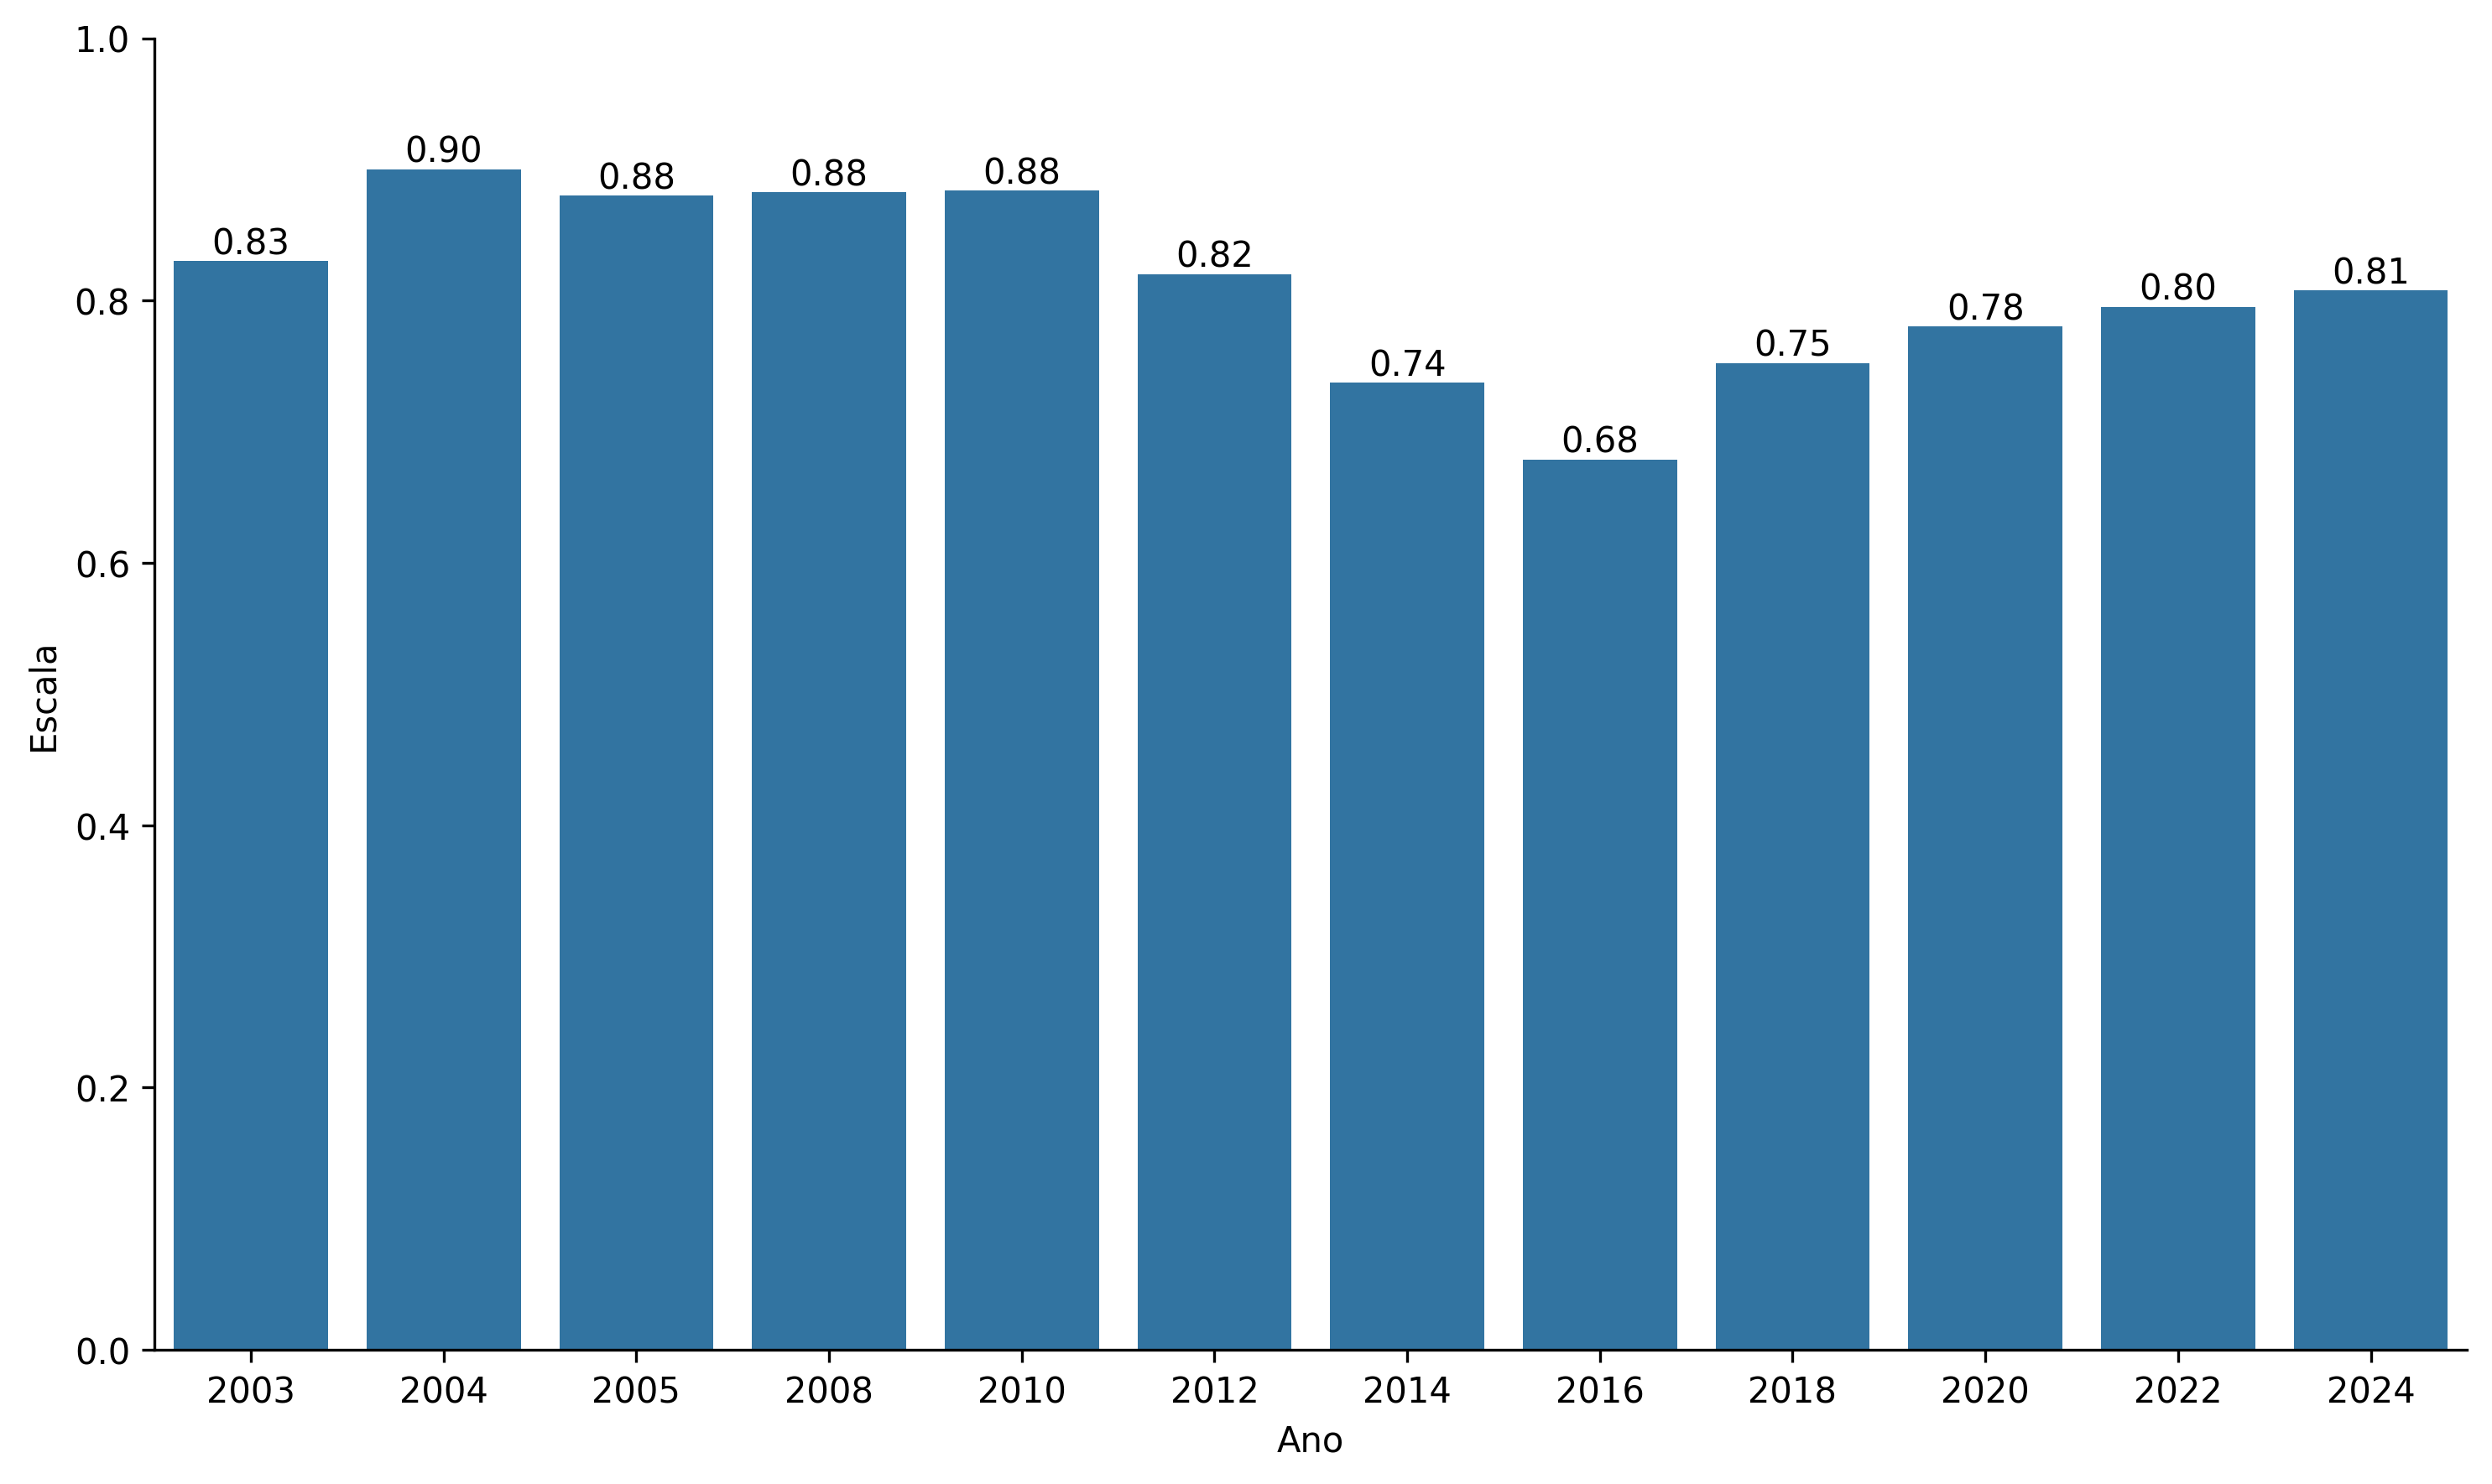
\includegraphics[width=1\linewidth]{figuras/egdi/egdi_brasil_hci.png}
    \label{fig:egdi_brasil_hci}
    \footnotesize{Fonte: baseado em \cite{ONU_edgi_mapa}.}
\end{figure}

\begin{figure}[H]
    \centering
    \caption{EGDI do Brasil: Telecommunication Infrastructure Index}
    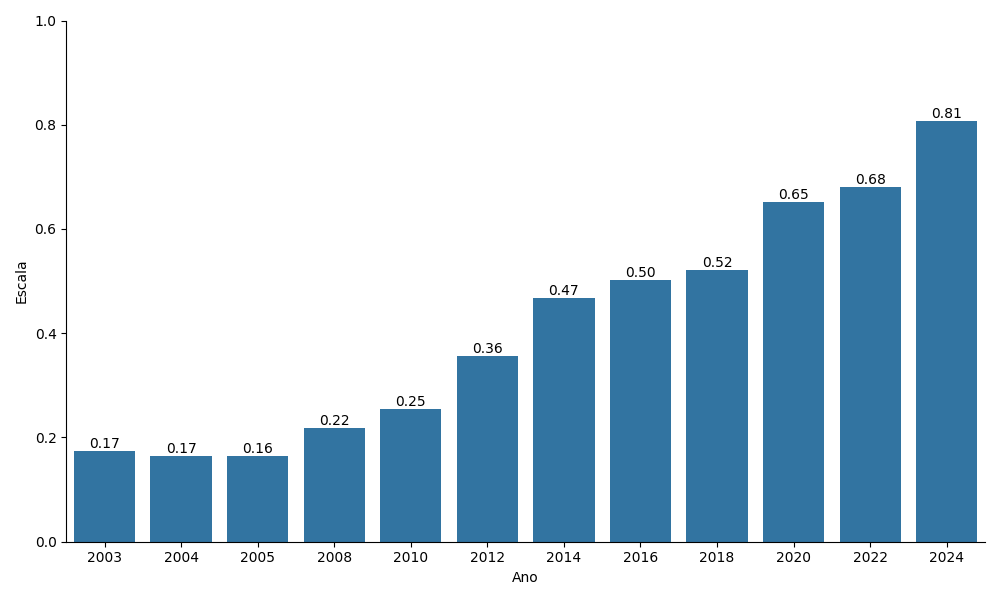
\includegraphics[width=1\linewidth]{figuras/egdi/egdi_brasil_tsi.png}
    \label{fig:egdi_brasil_tsi}
    \footnotesize{Fonte: baseado em \cite{ONU_edgi_mapa}.}
\end{figure}

\subsubsection{Indicadores de TIC de governo eletrônico}

A ONU tem \href{https://publicadministration.un.org/egovkb/en-us/Data/ICT-in-government}{indicadores de TIC de governo eletrônico} como algo complementar ao EGDI. Os indicadores são, conforme \cite{ONU_ICT_in_government_indicators}:

\begin{itemize}
    \item Existência de estratégia nacional de governo eletrônico ou equivalente;
    \item Existência de identidade digital para acessar ou outra forma de autencicação requirida para poder acessar serviços online;
    \item Existência de um portal de compras governamentais.
\end{itemize}

Os resultados globais dos indicadores estão presentes na figuras \ref{fig:national_government_strategy}, \ref{fig:national_identity} e \ref{fig:procurement_portal}.

\begin{figure}[H]
	\centering
	\caption{Indicador: Existência de estratégia nacional de governo eletrônico ou equivalente}
	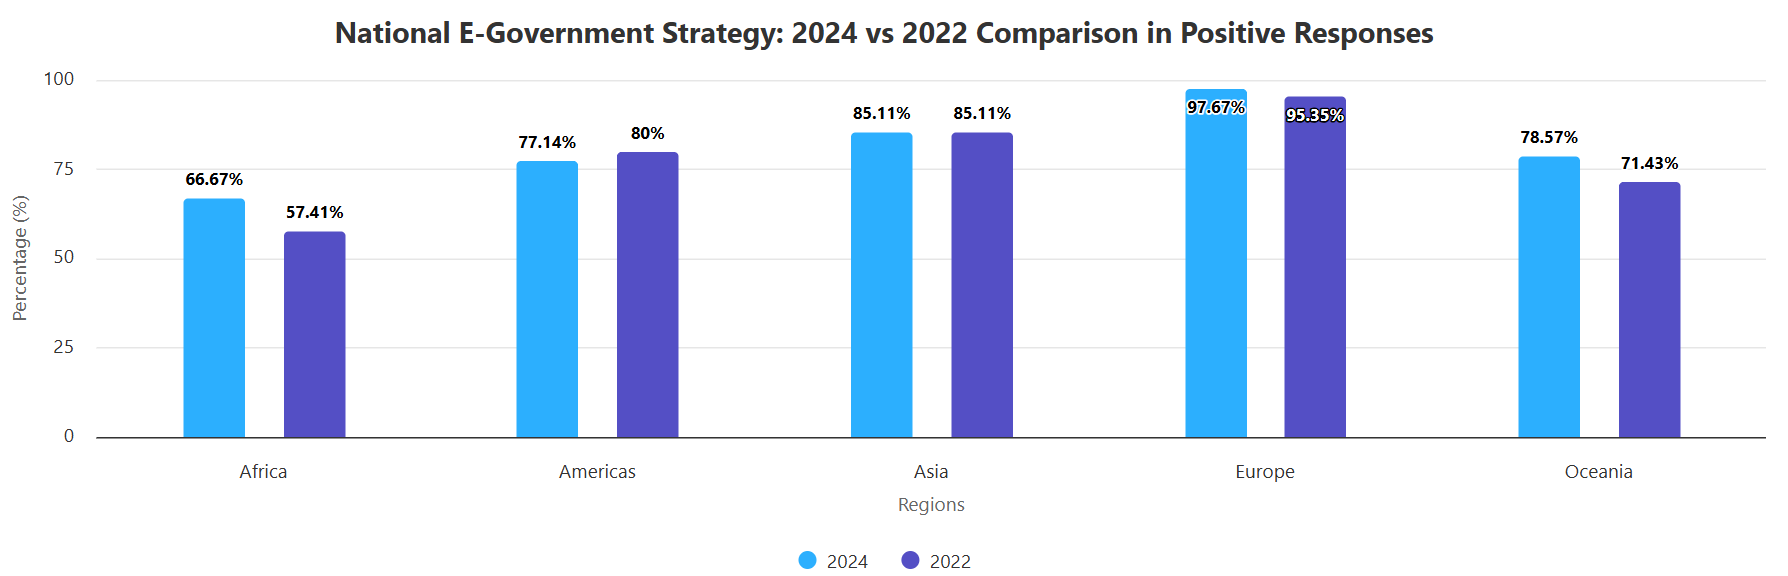
\includegraphics[width=1\linewidth]{figuras/ict_in_government/national_government_strategy}
	\label{fig:national_government_strategy}
	\footnotesize{Fonte: \cite{ONU_ICT_in_government_indicators}}
\end{figure}

\begin{figure}[H]
	\centering
	\caption{Indicador: Existência de identidade digital para acessar ou outra forma de autencicação requirida para poder acessar serviços online}
	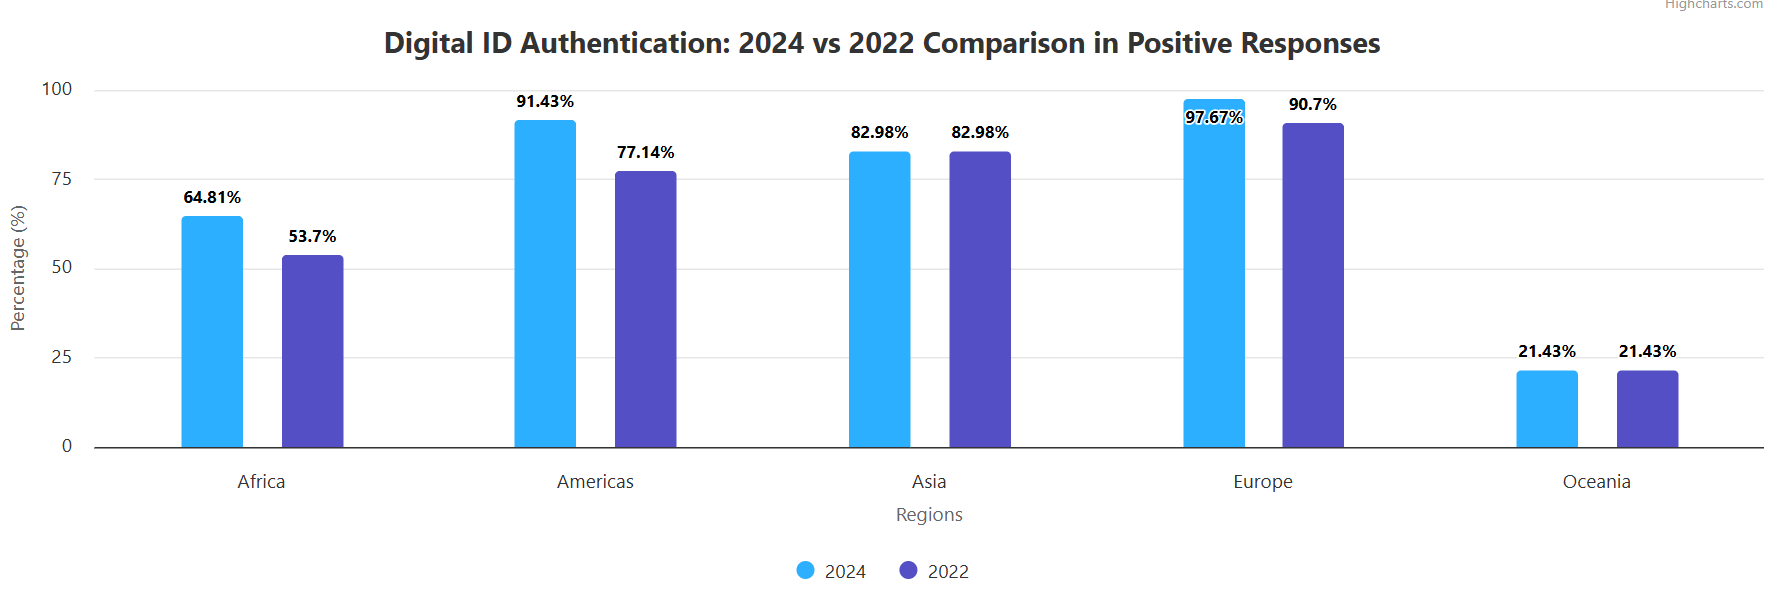
\includegraphics[width=1\linewidth]{figuras/ict_in_government/digital_identity}
	\label{fig:national_identity}
	\footnotesize{Fonte: \cite{ONU_ICT_in_government_indicators}}
\end{figure}

\begin{figure}[H]
	\centering
	\caption{Indicador: Existência de um portal de compras governamentais}
	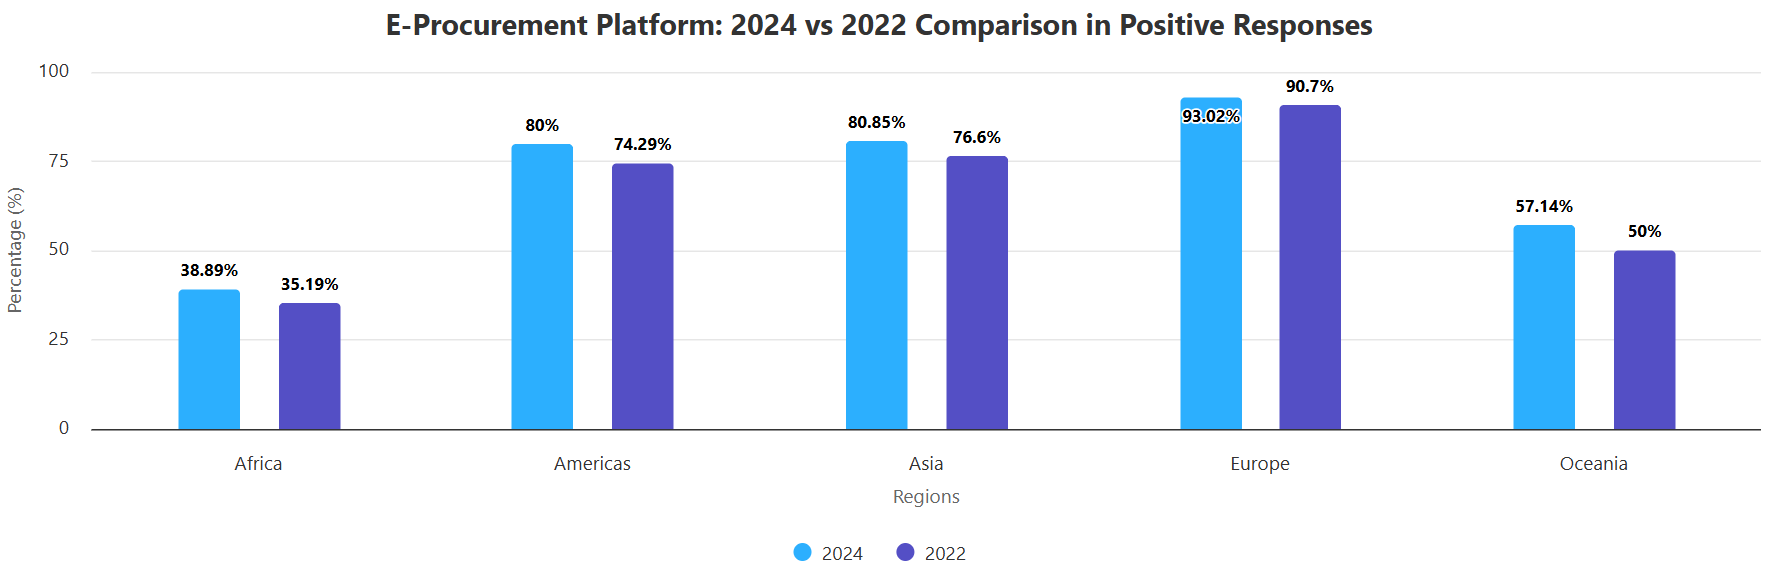
\includegraphics[width=1\linewidth]{figuras/ict_in_government/procurement_portal}
	\label{fig:procurement_portal}
	\footnotesize{Fonte: \cite{ONU_ICT_in_government_indicators}}
\end{figure}

Das três figuras, a Europa foi o continente cujos mais respondem que têm seguem os indicadores, superando os 90\%. A Oceania foi o continente que menos implementou políticas de identidade digital para acesso a serviços online. África e Oceania tiveram um desempenho ruim na implementação de portais de compra governamentais. O continente american apresentou bom desempenho nos três indicadores.
